\documentclass[twocolumn]{revtex4}

\usepackage{graphicx,epsfig}
\usepackage{amsmath}
\usepackage{amsfonts}
\usepackage{fancyhdr}
\usepackage{siunitx}


\begin{document}

\pagestyle{fancy}
\lhead{\bf Verifying open clusters using the Gaia catalogue}
\rhead{Daniel Monzonís Laparra}
\lfoot{Treball de Fi de Grau}
\rfoot{Barcelona, January 2018}


\title{Verifying open clusters using the Gaia catalogue}
\author{Author: Daniel Monzonís Laparra}
\affiliation{Facultat de Física, Universitat de Barcelona, Diagonal
645, 08028 Barcelona, Spain.}
\author{Advisor: Tristan Cantat-Gaudin}
%\date{\today}

\begin{abstract}
{\bf Abstract:} The aim of this work is to study several open clusters that have been previously identified, but using the newer and more precise data from the Gaia DR2 catalogue, trying to verify their existence, and determine their age and interstellar extinction.
\end{abstract}

\maketitle

%\tableofcontents


\section{Introduction}
Open clusters are groups of stars formed from the same molecular cloud simultaneously, and therefore the stars in the cluster share many properties like age, position, proper motion and composition. Because of this, many of these properties can be estimated much more easily from a cluster than from a single star. This information can then be used to trace the structure of the Milky Way, and makes open clusters very interesting for studying stellar evolution and stellar structure, since the only parameter that varies is the mass of each star.

Over 1200 open clusters have been identified within the Milky Way, but it is thought that there may exist around $10^5$ open clusters in the galaxy, since most open clusters form near the galactic plane, where the interstellar extinction is higher due to the higher amount of dust, making their observation much harder.

With the new release of data from Gaia, we can study open clusters with more precision than ever before. This data includes positions in the sky, proper motions, parallaxes, and magnitudes in three different photometric filters for over 1 billion stars.

Using the data from the UCAC4 catalogue, Sampedro et al.\cite{sampedro} reported the existence of 1876 open clusters, using three different membership methods. With the release of the Gaia DR2 catalogue, which contains more precise astrometric data, it is now possible to find and verify the existence of clusters more accurately.
There have already been attempts to identify open clusters using the Gaia DR2 catalogue, for instance, in the study of Cantat-Gaudin et al.\cite{cantat-gaudin}, 1269 clusters have been identified with the new data. Our first goal will be to crossmatch the data from both studies to find the clusters that haven't already been verified.

In this work, we will study some open clusters from both articles, focusing on clusters found in Sampedro's article but that have not been yet verified with the data from Gaia. We will also find estimates for the age and interstellar extinction of these clusters.


\section{The Gaia DR2 catalogue}
The second release of data from Gaia, the Gaia DR2 catalogue\cite{gaiadr2}, introduces high-precision measurements of various astrometry parameters, like proper motions and parallaxes, as well as photometric information for a total of $1 692 919 135$ sources. The catalogue contains a 5-parameter astrometric solution for over 1.3 billion stars, which include the position in the sky given by the right ascension and declination, the proper motion and the parallax. For the rest of the stars, which are the very faint ones ($G > 21$), a 2-parameter astrometric solution is given instead, with only the positions in the sky.

For bright stars ($G < 15$) the uncertainty in the positions and parallax is about $0.02-0.04\ \si{mas}$, and the uncertainty in the proper motions is about $0.07\ \si{mas.yr^{-1}}$. We will only be working with stars of at most $G = 17$, for which the uncertainty in the positions and parallax is of $0.1\ \si{mas}$ and of $0.2\ \si{mas.yr^{-1}}$ in the proper motions. Figure \ref{ppmxl_vs_gaiadr2} illustrates how this data is much more precise than what was available before, by comparing the proper motions of a well known cluster with the data from the PPMXL catalogue\cite{ppmxl} and Gaia DR2.

\begin{figure}[h!]
\centering
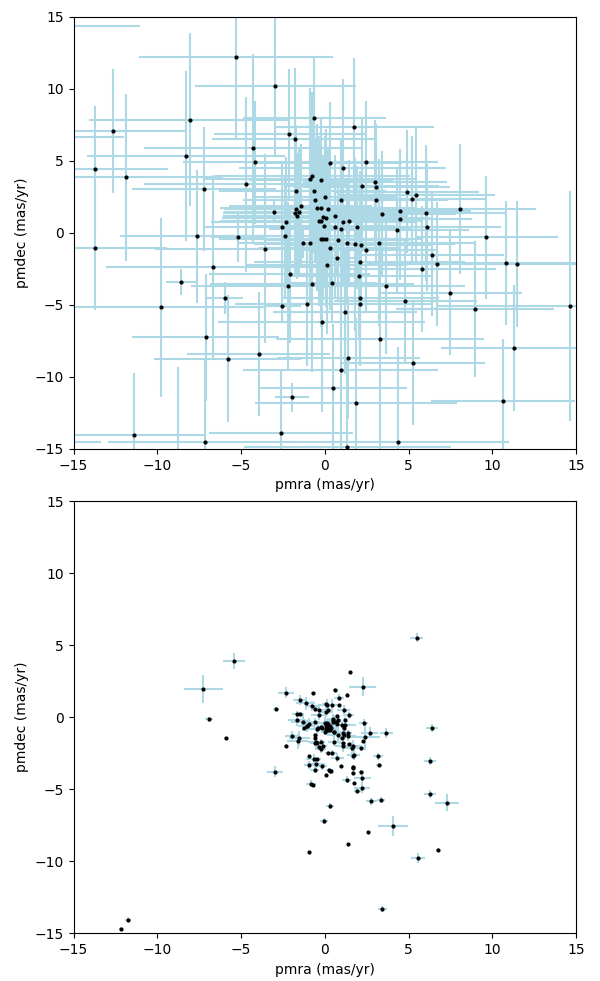
\includegraphics[scale=0.45]{ppmxl_vs_gaia_motions}
\caption{Comparison of the data from PPMXL and Gaia DR2 for the proper motions of the cluster Ivanov 2 \cite{ivanov}.}
\label{ppmxl_vs_gaiadr2}
\end{figure}


The catalogue also lists valuable information on the photometry of most of its sources on the $G$, $G_{BP}$ and $G_{RP}$ photometric passbands. This information will be very useful when determining the age of the clusters we will study, by using a colour-magnitude diagram.


\section{Identifying open clusters}

As a first measure to reduce the number of clusters that need to be verified, we will only check the clusters whose name is not present in the data from both studies. We end up with a list of 890 clusters, due mainly to naming inconsistencies and to the new study possibly missing some clusters found by the old one.

For each of these 890 clusters, we compute the mean right ascension and declination, which we will use as the center point of a circle with radius $\dfrac{\max(D) - \min(D)}{2}$ where $D$ is the set of declinations of each cluster. Then, we query the data from the Gaia DR2 catalogue for the region encompassed by this circle. We get stars with a magnitude $G < 17$, since the data from the UCAC4 catalogue does not show stars fainter than $G = 17$. This gives us the data for all the stars in the queried region, so we crossmatch this data with the data from the original study to leave only the stars that are supposedly part of the open cluster. To detect and filter the repeated cases due to name inconsistencies, the center positions of the already verified clusters are also added in the position plots.

\begin{figure*}
\centering
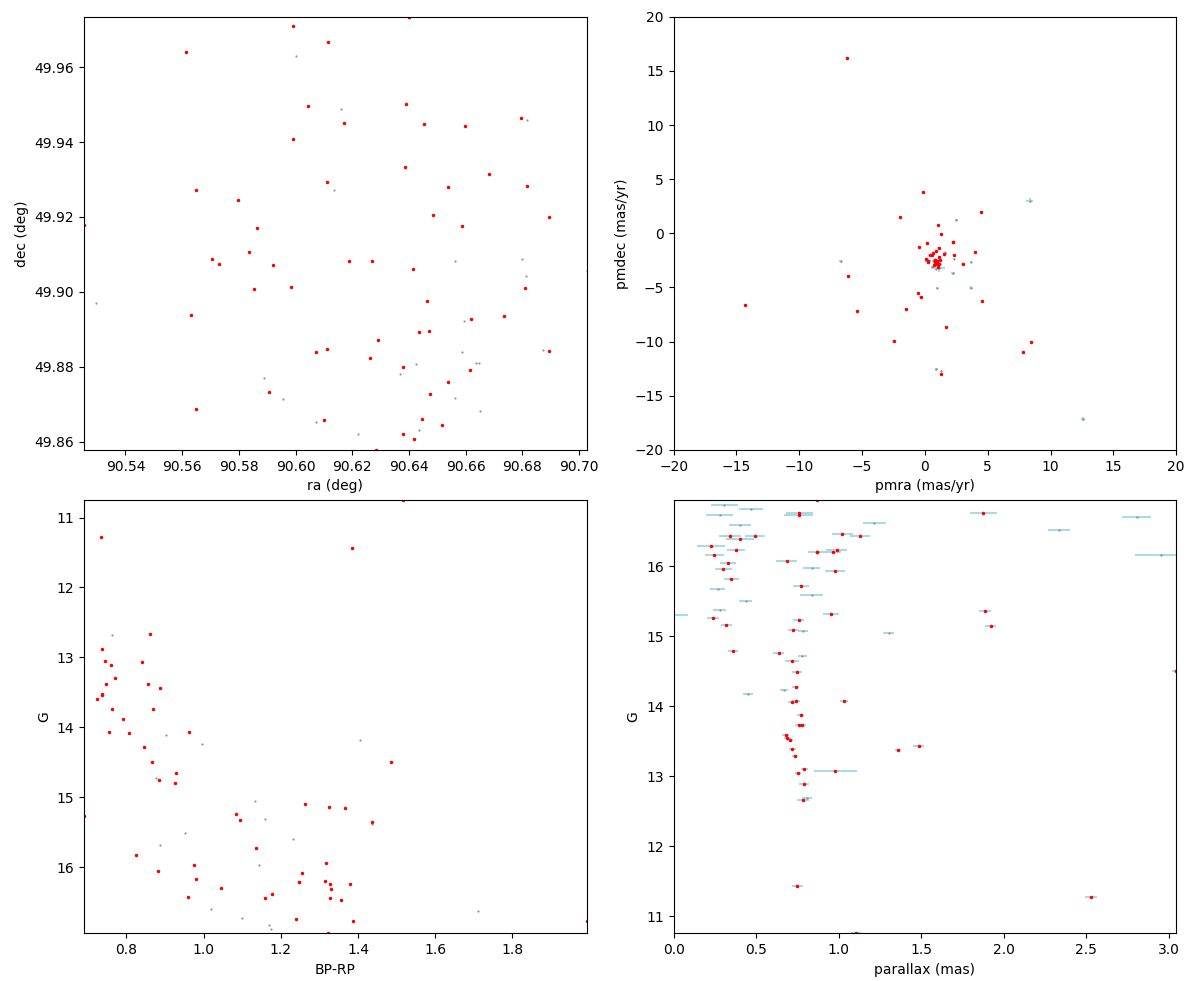
\includegraphics[scale=0.5]{NGC_2126_crossmatch}
\caption{Crossmatched data from the candidate cluster NGC 2126. The red dots correspond to stars from the Gaia DR2 catalogue that match to a star from Sampedro's study.}
\label{crossmatched_data}
\end{figure*}

Figure \ref{crossmatched_data} shows one example of the plots that were made for each of the clusters, for one of the cases that are confirmed to be a cluster and that will be studied in the next section to determine its age and interstellar extinction. Note that, in this case, the proper motion space is pretty compact, and there is a clear straight line in the parallax versus magnitude plot, showing that the stars are moving together and are at the same distance. In the color-magnitude diagram, we can see that some stars have already left the main sequence. We will study this in more detail in the following section.


\section{Determining the age and interstellar extinction of the cluster}
In this section we discuss the procedure followed to determine an approximation of the age and interstellar extinction of some clusters. We try this method for a total of 14 clusters, some of which are taken from the list of verified clusters in the study of Cantat-Gaudin, and the rest are cases from the study of Sampedro which we have verified in the previous section. The complete list of tested clusters, as well as some data on them, can be found in Table \ref{tab:clusters}. %TODO comment on the method used to get the members of the cluster
Note that a lower parallax means a greater distance.

%TODO fill with data
\begin{table}[h!]
\begin{tabular}{|l|c|c|c|}
\hline
\textbf{Cluster} & \textbf{Position (deg)} & \textbf{Parallax (mas)} & \textbf{Members} \\
\hline
Alessi 3 & $(109.95, -46.05)$ & $3.5619$ & $243$ \\
\hline
Collinder 421 & $(305.83, 41.69)$ & $0.8169$ & $283$ \\
\hline
ESO 332 08 & $(253.80, -40.96)$ & $0.5332$ & $417$ \\
\hline
Herschel 1 & $(116.72, 0.15)$ & $3.3385$ & $149$ \\
\hline
NGC 752 & $(29.24, 37.77)$ & $2.2245$ & $263$ \\
\hline
NGC 1039 & $(40.51, 42.74)$ & $1.9350$ & $659$ \\
\hline
NGC 2126 & $(90.65, 49.91)$ & $0.7490$ & $151$ \\
\hline
NGC 2169 & $(92.12, 13.94)$ & $0.9863$ & $133$ \\
\hline
NGC 2287 & $(101.51, -20.70)$ & $1.3503$ & $673$ \\
\hline
NGC 2360 & $(109.44, -15.63)$ & $0.8994$ & $695$ \\
\hline
NGC 2479 & $(118.76, -17.73)$ & $0.6311$ & $159$ \\
\hline
Ruprecth 8 & $(105.41, -13.56)$ & $0.4278$ & $138$ \\
\hline
Stock 6 & $(35.93, 63.79)$ & $0.9536$ & $144$ \\
\hline
Berkeley 100 & $(351.48, 63.78)$ & $0.1461$ & $57$ \\
\hline
\end{tabular}
\caption{List of clusters that have been studied, and their mean position (given in (ra, dec)) and mean parallax, computed using the data from Gaia DR2, and the number of member stars of the cluster.} %TODO mention method name
\label{tab:clusters}
\end{table} 

\section{Problems when fitting isochrones}
\subsection{Blue stragglers}
Talk about blue stragglers, show some plots where they clearly appear...

\subsection{Binary sequences}
Talk about binary sequences due to binary stars.

\subsection{Differential extinction}
Talk about how extinction can change a lot even within the same cluster. Show an example where this happens, where more distant stars have more extinction (we saw one example with Tristan).

\section{Conclusions}


\section{Appendix}


\vspace*{0.5cm}
\begin{acknowledgments}

\end{acknowledgments}


\begin{thebibliography}{99}

\bibitem{sampedro} Sampedro L., Dias W. S., Alfaro E. J., Monteiro H., and Molino A., (2017), arXiv:1706.05581 [astro-ph.SR].

\bibitem{cantat-gaudin} Cantat-Gaudin T. et al., (2018), arXiv:1805.08726 [astro-ph.GA]

\bibitem{star-clusters} K. Janes, \textsl{Star Clusters}, Encyclopedia of Astronomy and Astrophysics, (Nature Publishing Group, 2001)

\bibitem{gaiadr2} A.G.A. Brown, A. Vallenari, T. Prusti et al., (2018), arXiv:1804.09365 [astro-ph.GA]

\bibitem{ppmxl} S. Roeser, M. Demleitner and E. Schilbach, (2010), arXiv:1003.5852 [astro-ph.GA]

\bibitem{ivanov} A. L. Tadross, R. Bendary, (2014), arXiv:1403.3014 [astro-ph.GA]


\end{thebibliography}


\end{document}
